\documentclass{article} % For LaTeX2e
\usepackage{nips13submit_e,times}
\usepackage{hyperref}
\usepackage{url}
\usepackage{graphicx}
\usepackage{amsmath}
\usepackage{amsfonts}
\usepackage{ upgreek }
\usepackage{subfigure}
\usepackage{algorithm}
\usepackage{placeins}
\usepackage{algpseudocode}
\usepackage{tkz-graph}
\usetikzlibrary{arrows}
%\usepackage{amsmath}
%\usepackage{amssymb}
%\usepackage{package}
%\usepackage{graphicx}
%\usepackage[utf8]{inputenc}  
%\usepackage[T1]{fontenc} 
%\usepackage[top=1cm,bottom=1cm,left=0.5cm,right=1.5cm,asymmetric]{geometry}
%\usepackage{amsfonts}
%\usepackage{graphicx}
%\usepackage{amsmath}
%\usepackage{caption}
%\usepackage{subcaption}
%\usepackage{float}
%\usepackage{subfig}
%\usepackage{fancyhdr}
%\documentstyle[nips13submit_09,times,art10]{article} % For LaTeX 2.09


\title{Significant perturbations in observability graph}

\author{
Oussama Ennafii\\
Master MVA\\
ENS Cachan\\
\texttt{oennafii@ens-cachan.fr} \\
\And
Sammy Khalife \\
Master MVA\\
ENS Cachan\\
\texttt{skhalife@ens-cachan.fr}
}

% The \author macro works with any number of authors. There are two commands
% used to separate the names and addresses of multiple authors: \And and \AND.
%
% Using \And between authors leaves it to \LaTeX{} to determine where to break
% the lines. Using \AND forces a linebreak at that point. So, if \LaTeX{}
% puts 3 of 4 authors names on the first line, and the last on the second
% line, try using \AND instead of \And before the third author name.

\newcommand{\fix}{\marginpar{FIX}}
\newcommand{\new}{\marginpar{NEW}}

%\nipsfinalcopy % Uncomment for camera-ready version
\bibliographystyle{plain}
\begin{document}


\maketitle

\begin{abstract}
Following the work on Online Learning with feedback graphs \cite{journals/corr/AlonCDK15} ,
we investigate the case of unstable graphs (even a small change in the graph structure like deleting or adding one edge can change the regret of the algorithm significantly), and design experiments which show the difference of the regret of the original and perturbed graph.
\end{abstract}

\section*{1 Introduction}
Given a feedback graph of observation, and a sequence of losses $(l_t)_{1 \leq t \leq T}$, let us denote $S$ the set of all strategies which have as output the sequence of actions $(I_t)_{1 \leq t \leq T}$. We denote the minimax regret by 
$$ R(G,T)=\min_{S} \max_{l_1,...,l_T} \mathbb{E}  \sum_{t=1}^{T} l_t(I_t) -\min_{i} \sum_{t=1}^{T}l_t(i)  $$
Which represents the best strategy answer to the worst case scenario in terms of loss sequence.
In [1], this minimax regret has been shown to be bounded with respect to the geometry of the feedback graph.~\\
~\\
If the graph is strongly observable with independence number $\alpha$, then 
$ R(G,T) = \tilde{\Uptheta}(\alpha^{1/2}T^{1/2})$.
If the graph is weakly observable with domination number $\delta$, then 
$ R(G,T) = \tilde{\Uptheta}(\delta^{1/2}T^{1/2})$
If the graph is unobservable, then 
$ R(G,T) = \tilde{\Uptheta}(T) $.

Similar to the EXP3 in the contex of adversarial bandits, the EXP3G algorithm [1] explores the graph given an exploration set U, an exploration rate $\gamma \in [0,1]$ and a learning rate $\eta > 0$. U(V) is the uniform distribution over V.

 \FloatBarrier
 \begin{algorithm}
 	\caption{EXP3G algorithm}\label{RS}
 	for t=1,...,T ~\\
 	Draw $ I_t \sim p_t = (1-\gamma)q_t + \gamma u(V) $ ~\\
 	Incure loss $l_t(I_t)$ and with respect to the feedback graph, observe $\{(i,l_t(i)), i \in N^{out}(I_t)\}$ ~\\
 	Update estimators and distribution :
 	$\hat{l}_{t}(i)=\frac{l_t(i)}{P_{t}(i)} \textbf{1}_{\{ i \in N^{out}(I_t)\}} \qquad$ $P_t(i)=\sum_{j \in N^{in}(i)}p_{t}(j)$, 
 	$q_{t+1}(i)=\frac{q_t(i)exp(-\eta \hat{l}_{t}(i))}{\sum_{j \in V}q_t{j}exp(-\eta \hat{l}_{j}(i))}$~\\
 	end
 \end{algorithm}
 \FloatBarrier
 
\section*{2 Unstable graphs}
~\\
Blablabla
~\\
\section*{3 Experiments }




\SetVertexNormal[Shape      = circle,
FillColor  = white,
LineWidth  = 2pt]
\SetUpEdge[lw         = 1.5pt,
color      = black,
labelcolor = white,
labeltext  = red,
labelstyle = {sloped,draw,text=blue}]


\begin{figure}[h]
	
\subfigure[before]{
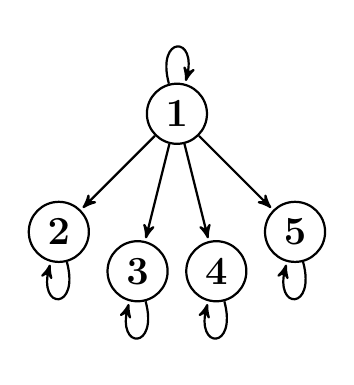
\begin{tikzpicture}[->,>=stealth',shorten >=1pt,auto,node distance=3cm,
thick,main node/.style={circle,draw,font=\Large\bfseries}]
\node[main node] (1) at (0,0) {1};
\node[main node] (2) at (-1.5,-1.5) {2};
\node[main node] (3) at (-0.5, -2) {3};
\node[main node] (4) at (0.5,-2) {4};
\node[main node] (5) at (1.5,-1.5) {5};
\path
(1) edge [loop above] node {} (1);
\path
(2) edge [loop below] node {} (2);
\path
(3) edge [loop below] node {} (3);
\path
(4) edge [loop below] node {} (4);
\path
(5) edge [loop below] node {} (5);
%edge [bend right] node {0.4} (2)
%(1) edge node [below]{} (2)
%%(1) edge [loop below] node {} (3)
%%edge node[right] {0.1} (1)
%(1) edge node[below] {} (3); 
%(1) edge node[below] {} (4);
%(1) edge node[below] {} (5);    
\draw (1) -- (2);
\draw (1) -- (3);
\draw (1) -- (4);
\draw (1) -- (5); 
\end{tikzpicture} }
\hfill
\subfigure[after]{
	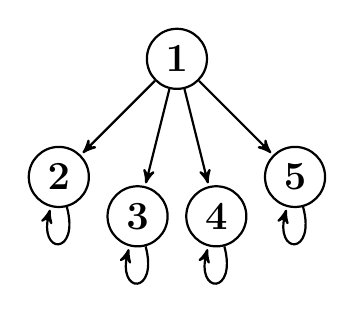
\begin{tikzpicture}[->,>=stealth',shorten >=1pt,auto,node distance=3cm,
	thick,main node/.style={circle,draw,font=\Large\bfseries}]
	
	\node[main node] (1) at (0,0) {1};
	\node[main node] (2) at (-1.5,-1.5) {2};
	\node[main node] (3) at (-0.5, -2) {3};
	\node[main node] (4) at (0.5,-2) {4};
	\node[main node] (5) at (1.5,-1.5) {5};
	%\path
	%(1) edge [loop above] node {} (1);
	\path
	(2) edge [loop below] node {} (2);
	\path
	(3) edge [loop below] node {} (3);
	\path
	(4) edge [loop below] node {} (4);
	\path
	(5) edge [loop below] node {} (5);
	%edge [bend right] node {0.4} (2)
	%(1) edge node [below]{} (2)
	%%(1) edge [loop below] node {} (3)
	%%edge node[right] {0.1} (1)
	%(1) edge node[below] {} (3); 
	%(1) edge node[below] {} (4);
	%(1) edge node[below] {} (5);    
	\draw (1) -- (2);
	\draw (1) -- (3);
	\draw (1) -- (4);
	\draw (1) -- (5);
\end{tikzpicture} }
\end{figure}
%\caption{Revealing action graph (strongly observable)} \label{fig:M1}







\bibliography{references.bib}

\end{document}
